\documentclass{article}

\usepackage[final]{neurips_2024}



\usepackage[utf8]{inputenc} % allow utf-8 input
\usepackage[T1]{fontenc}    % use 8-bit T1 fonts
\usepackage{hyperref}       % hyperlinks
\usepackage{url}            % simple URL typesetting
\usepackage{booktabs}       % professional-quality tables
\usepackage{amsfonts}       % blackboard math symbols
\usepackage{nicefrac}       % compact symbols for 1/2, etc.
\usepackage{microtype}      % microtypography
\usepackage{xcolor}         % colors
\usepackage{amsmath}
\usepackage{graphicx}
\usepackage{pythonhighlight}
\usepackage{subcaption}
\usepackage{float}
\usepackage{makecell}
\usepackage[symbol]{footmisc}
\usepackage{algpseudocodex}
\graphicspath{{Images/}}
\usepackage{cite}
\usepackage[numbers]{natbib}


\hypersetup{colorlinks=true,linkcolor=blue, linktocpage}

\newcommand{\todo}[1]{\textcolor{red}{#1}}

\newcommand{\R}{\mathbb{R}}
\newcommand\Tstrut{\rule{0pt}{2.6ex}}

\title{Neural Network and Optimizers}


\author{
  Sahil Chaudhary^* \\
  \And
  Om Prakash Chaudhary^* \\
  \And
  Pratham Gupta^* \\
  \And
  Rolla Siddartha^*\\
  \And
  Aditya Manjunatha^*\\
  \And
  Adithya K Anil^*
  % \And
  % Bachelor of Technology \\
  % Indian Institute of Science\\
  % \texttt{\{sahilc,\}@iisc.ac.in}
}

\begin{document}


\maketitle

\def\thefootnote{*}\footnotetext{All authors contributed equally to this work.}
\def\thefootnote{\arabic{footnote}}

\begin{abstract}
Neural networks have revolutionized machine learning by surpassing traditional models such as Support Vector Machines (SVM). However, the performance of neural networks is heavily dependent on the optimization methods used to update their weights and biases. In this paper, we provide a comprehensive comparison of four prominent optimization algorithms: Stochastic Gradient Descent (SGD), Momentum, RMSProp, and Adam. We detail the mathematical foundations and algorithms for each method and offer practical guidelines for implementing neural networks from scratch. Using the MNIST and CIFAR-10 datasets, we empirically evaluate the performance of these optimizers. Our results demonstrate that Adam consistently outperforms other stochastic optimization methods, providing faster convergence and higher accuracy. This paper aims to serve as a valuable resource for beginners and practitioners in the field of neural network optimization.
\end{abstract}
\input{introduction}

\input{sgd}

\section*{Momentum}
% Abstract regarding Momentum - Adithya K Anil
Momentum optimizer is an optimization algorithm which accelerates the process of gradient descent by considering the previous gradients to smooth out the updates. By considering the accumulated gradients, momentum can help the optimizer to accelerate in directions with persistent gradients, leading to faster convergence. The momentum optimizer introduces a velocity term v which denotes the accumulated gradient. The consideration of velocity term also help in smoothing out noises as well as escaping shallow local minimas by carrying the optimizer forward. \\
\textbf{Hyperparameters: }
\begin{itemize}
    \item \textbf{Learning Rate} ($\eta$): Controls the size of the steps the optimizer takes in the direction of the negative gradient in each loop. It affects how fast or slow the model learns (usually in between 0.001 to 0.1)
    \item \textbf{Momentum Coefficient} ($\gamma$): Controls the contribution of the past gradients to the current update. A higher momentum coefficient means that more of the previous gradients are included, which can help to smooth the updates and accelerate convergence (usually in between 0.8 to 0.99)
\end{itemize}
\textbf{Algorithm: }
\begin{itemize}
    \item \textbf{Initilization}:
    \begin{itemize}
        \item Parameters: Initialize the parameters(weights) of the model, either as a zero matrix or randomly. ( It is preferred to initialize it randomly )
        \item Hyperparameters : Initialize the hyperparameters so a value in the typical range however these values can be modified later depending on need.    
    \end{itemize}
    \item \textbf{Loop:}
    \begin{enumerate}
        \item Calculate the gradient : In each iteration, compute the gradient of the loss function with respect to each of the parameters. If the parameters are $\theta_t$, cost function is $J(\theta$), where subscript $t$ denotes the iteration, then the gradient $g_t = \nabla_{\theta} J(\theta_t)$
        \item Update Velocity recursively : 
        $v_t = \gamma v_{t-1} + \eta g_t$
        \item Update Parameters recursively :
        $\theta_t = \theta_{t-1} - v_t$
    \end{enumerate}
\end{itemize}
    
\newpage


\section*{Root Mean Square Propogation}
The RMSProp optimizer is one which is used in specific scenarios, where the Vanilla SGD and SGD with Momentum take a lot of iterations to converge to the minima of the loss function. The main feature of this optimizer is that it is able to adapt the learning rate separately for each parameter(weights) of the model. Note that this is not the only optimizer that uses this idea of adaptive gradients.

\subsection*{Hyperparameters}
\begin{itemize}
    \item \textbf{Learning Rate} ($\alpha$): Controls the step size during the parameter update.
    \item \textbf{($\beta$):} : Controls how influential the past velocities will be in the current update ( Usually kept as 0.9 )
    \item \textbf{Epsilon} ($\epsilon$): A small constant to prevent division by zero (e.g., $10^{-8}$).
\end{itemize}

\textbf{Algorithm: }
\begin{itemize}
    \item \textbf{Initilization}:
    \begin{itemize}
        \item Parameters: Initialize the parameters(weights) of the model, either as a zero matrix or randomly. ( It is preferred to initialize it randomly )
        \item Hyperparameters : Initialize the hyperparameters so a value in the typical range however these values can be modified later depending on need.    
    \end{itemize}
    \item \textbf{Loop:}
    \begin{enumerate}
        \item Update Velocity recursively : 
        $v_(t+1) = \beta v_{t} + (1 - \beta )\nabla W_t^2$
        \item Update Parameters recursively :
        $W_{t+1} = W_{t} - \alpha \frac{\nabla W_t}{\sqrt{V_{t+1} + \epsilon}}$
    \end{enumerate}
\end{itemize}

\section*{Adam}
% Abstract regarding ADAM
ADAM algorithm is an optimization technique that combines the advantages of two other popular optimization algorithms AdaGrad and RMSProp. ADAM is able to achieve a variable learning rate for each parameter independently by utilizing first and second moments allowing it to achieve convergence faster and optimize for all parameters simultaneously.  \\
\\

% Hyper parameters and there uses
\textbf{Hyperparameters:}
\begin{itemize}
    \item \textbf{Learning Rate} ($\alpha$): Controls the step size during the parameter update.
    \item \textbf{Decay Rates for the moment estimates:}
    \begin{itemize}
        \item $\beta_1$: Exponential decay rate for the first moment estimates (usually close to 1, e.g., 0.9).
        \item $\beta_2$: Exponential decay rate for the second moment estimates (usually close to 1, e.g., 0.999).
    \end{itemize}
    \item \textbf{Epsilon} ($\epsilon$): A small constant to prevent division by zero (e.g., $10^{-8}$).
\end{itemize}

\newpage



% Full Mathematics 
\textbf{Algorithm:}
\begin{itemize}
    \item \textbf{Initialization}:
    \begin{itemize}
        \item \textbf{Parameters}: Initialize parameters (weights) of the model, typically randomly.
        \item \textbf{Moment Estimates}: Initialize the first moment (mean) $m_0 = 0$ and the second moment (uncentered variance) $v_0 = 0$.
    \end{itemize}

    \item \textbf{Loop}:
    \begin{enumerate}
  
        \item \textbf{Gradient Computation}:
        \begin{itemize}
            \item At each time step $t$, compute the gradient of the loss function with respect to the parameters $\theta_t$: $g_t = \nabla_{\theta} J(\theta_t)$.
        \end{itemize}
    
        \item \textbf{Update Biased First Moment Estimate}:
        \begin{itemize}
            \item $m_t = \beta_1 \cdot m_{t-1} + (1 - \beta_1) \cdot g_t$
        \end{itemize}
    
        \item \textbf{Update Biased Second Moment Estimate}:
        \begin{itemize}
            \item $v_t = \beta_2 \cdot v_{t-1} + (1 - \beta_2) \cdot g_t^2$
        \end{itemize}
    
        \item \textbf{Compute Bias-Corrected First Moment Estimate}:
        \begin{itemize}
            \item $\hat{m}_t = \frac{m_t}{1 - \beta_1^t}$
        \end{itemize}
    
        \item \textbf{Compute Bias-Corrected Second Moment Estimate}:
        \begin{itemize}
            \item $\hat{v}_t = \frac{v_t}{1 - \beta_2^t}$
        \end{itemize}
    
        \item \textbf{Parameter Update}:
        \begin{itemize}
            \item Update the parameters $\theta_t$ using the corrected estimates:
            \[
            \theta_t = \theta_{t-1} - \alpha \cdot \frac{\hat{m}_t}{\sqrt{\hat{v}_t} + \epsilon}
            \]
        \end{itemize}

    \end{enumerate}
\end{itemize}

% Special notes:

Bias Correction in necessary in intial stages of algorithm as $\beta_1$ and $\beta_2$ are close to $1$ and $m_0$ and $v_0$ are initialized to 0 , effect of gradients will be significantly reduced at beginning if bias correction is not performed. \\
In the later stages as $\beta_1^t$ and $\beta_2^t$ tends to 0 bias correction is insignificant. 

% Advantages and Disadvantages 





\section*{Experiments}
We compared the performance of all the learning algorithms over MNIST dataset with simple dense neural network architecture. Our network had an input layer with 28*28 (784) input features which correspond to pixel brightness of greyscale digits followed by a hidden layer with 50 features and ReLU activation and an output layer with 10 features with Softmax activation corresponding to the probability of digit.

For a fair comparison between all the learning algorithms, we ran each algorithm with various values of hyperparameter, with fixed initial weights and bias initialization. This helped us to choose the best hyperparameter values based on model architecture, irrespective of random initialization.
\begin{figure}[H]
    \centering
    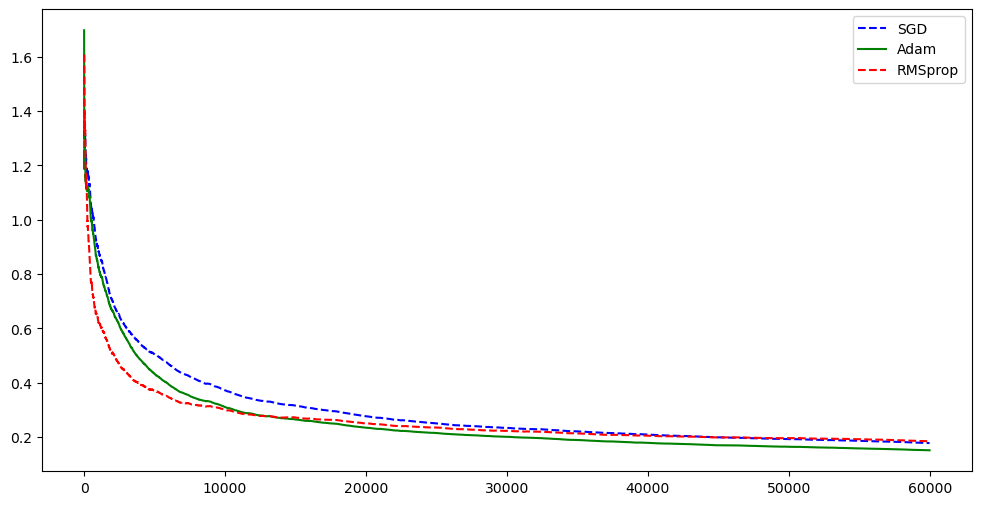
\includegraphics[width=0.7\linewidth]{Images/MSE Learning Curve.png}
    \caption{MSE vs Iteration (Best Parameters)}
\end{figure}
The above figure shows MSE Learning Curve on MNIST Dataset. All the algorithms were trained for 1 epoch over the entire dataset. Although RMSprop had fast initial learning rate, adam outperformed it shortly and converged to a lower MSE value.
The best parameters were found by running the algorithms with different parameters and choosing the best-performing parameter.
\begin{figure}[H]
    \centering
    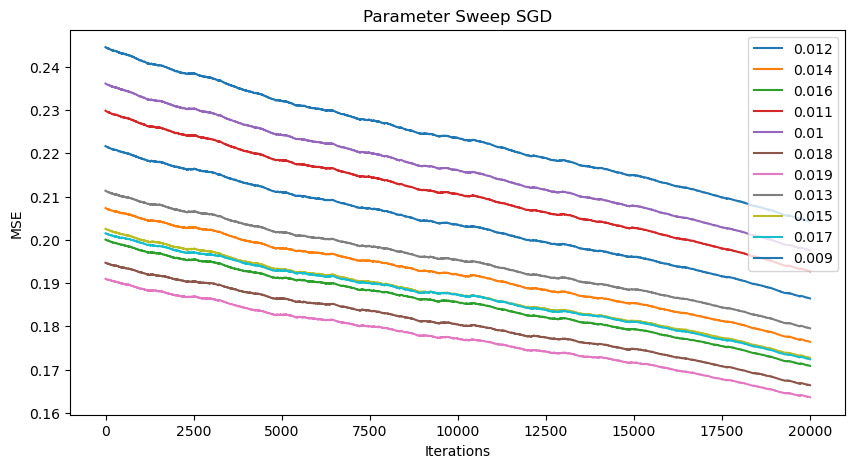
\includegraphics[width=0.7\linewidth]{Images/SGD_sweep.png}
    \caption{Stepsize Sweep for SGD (Optimal step size 0.019)}
\end{figure}
With step size 0.019, SGD consistently had an accuracy of about $91-93\%$ on the test set when trained for 1 Epoch.
\begin{figure}[H]
    \centering
    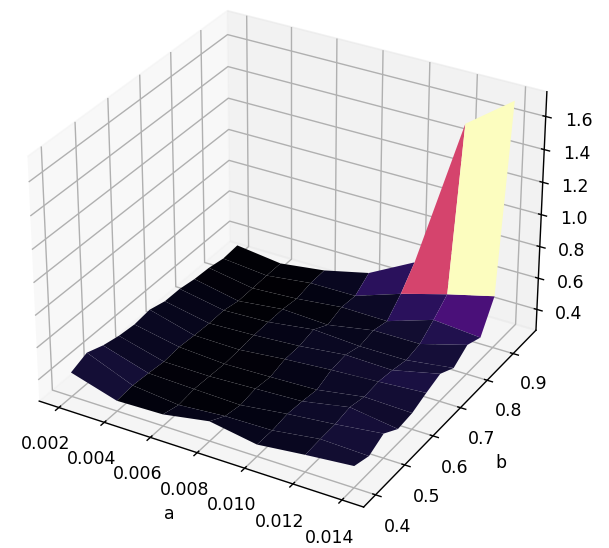
\includegraphics[width=0.7\linewidth]{Images/a_b_MSE_RMSprop.png}
    \caption{Stepsize(a) vs Moment Estimate(b) vs MSE for RMSprop}
\end{figure}
RMSprop works good over a range of parameter values. We used Stepsize(a) = 0.006 and  Moment Estimate(b) = 0.6 and it had an accuracy of about $91-93\%$ on the test set when trained for 1 Epoch.
\newpage
\begin{figure}[H]
    \centering
    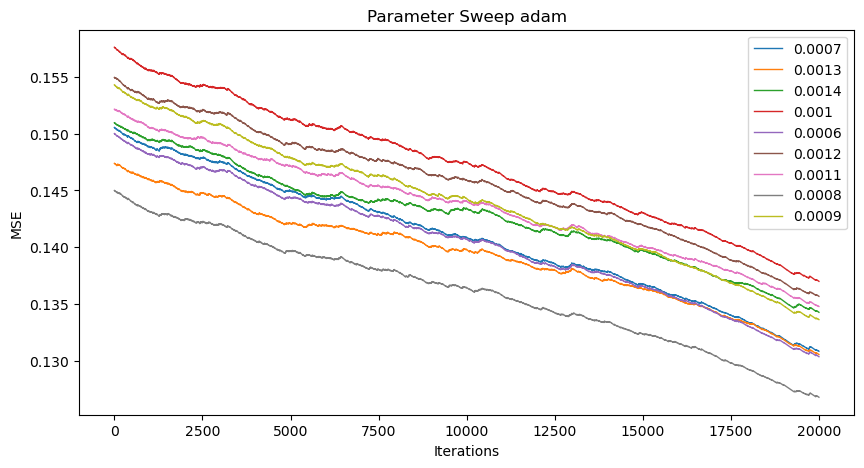
\includegraphics[width=0.7\linewidth]{Images/adam_sweep.png}
    \caption{Stepsize sweep for Adam}
\end{figure}
\begin{figure}[H]
    \centering
    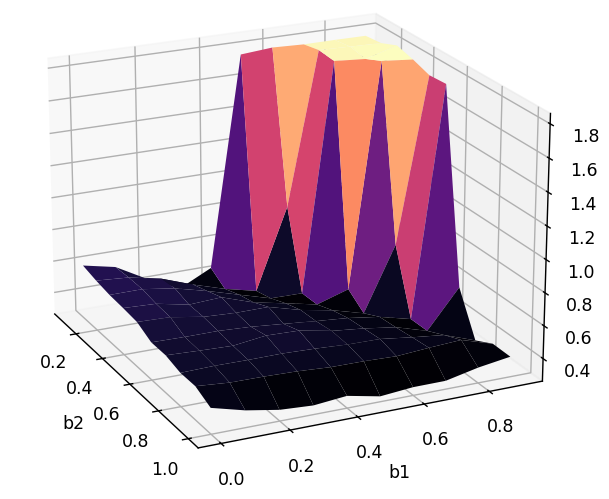
\includegraphics[width=0.7\linewidth]{Images/b1_b2_ MSE_adam.png}
    \caption{Moment Estimate Parameters b1 vs b2 vs MSE Adam}
    \label{fig:enter-label}
\end{figure}
Adam performs well for small steps size close to 8e-4. Here we ran the algorithm with various stepsize and Moment Estimate Parameters fixed to b1 = 0.9 and b2 = 0.999. Changing the Moment Estimate Parameters slightly produced similar result. Adam moment estimate parameters work well over a range of values but the best parameter values among all are b1 = 0.5 and b2 = 0.999. The parameters produced accuracy of about $93-95\%$ on the test set when trained for 1 Epoch.

\newpage
\section*{Conclusions}
In this paper, we conducted a comparison of various optimization algorithms including SGD,Momentum, RMSProp, and Adam\citep{kingma2014adam}, to evaluate their performance in training in neural networks. We analyzed each optimizer's convergence behaviour and sensitivity to hyperparameters using visualisations of the MSE over iterations. Our results showed that the \textbf{Adam optimizer} consistently outperformed other methods across different hyperparameter settings, achieving the fastest convergence and the lowest MSE values on the MNIST Dataset\citep{lecun2010mnist}.

Our findings confirm that while the choice of optimizer significantly impacts convergence speed and final accuracy, Adam \citep{ho2019flow} provides a more efficient and reliable solution for neural network training, especially in large-scale settings. This conclusion serves as a guide for practitioners in selecting appropriate optimizers for deep learning applications, encouraging further exploration into hybrid optimizers that can achieve even better performance.

\bibliographystyle{plain}
\bibliography{cite}

\end{document}